\newpage{}

\begin{landscape}

\hypertarget{results-per-algorithm}{%
\section{Results Per Algorithm}\label{results-per-algorithm}}

\subsection{Overview}

\begin{tabular}{lllrr}
\hline
 Algorithm   & Training on   & Estimating    &   with params &                 deviation \\
\hline
 A001        & SWEArchiv2020 & SWEArchiv2020 &         25\%P &  -1.277 $\pm$ 6.822 hours \\
 A001        & SWEArchiv2020 & SWEArchiv2020 &         50\%P &  -0.900 $\pm$ 6.369 hours \\
 A001        & SWEArchiv2020 & SWEArchiv2020 &         75\%P &   0.099 $\pm$ 6.097 hours \\
 A001        & SWEArchiv2020 & SWEArchiv2020 &         80\%P &   0.453 $\pm$ 5.573 hours \\
 A001        & SWEArchiv2020 & SWEArchiv2020 &         90\%P &   2.057 $\pm$ 5.626 hours \\
 A001        & SWEArchiv2020 & SWEArchiv2020 &        100\%P &  -1.829 $\pm$ 7.691 hours \\
 A001        & SWEArchiv2020 & SWEArchiv2021 &         25\%P & -1.546 $\pm$ 12.133 hours \\
 A001        & SWEArchiv2020 & SWEArchiv2021 &         50\%P & -1.320 $\pm$ 12.129 hours \\
 A001        & SWEArchiv2020 & SWEArchiv2021 &         75\%P & -0.675 $\pm$ 12.127 hours \\
 A001        & SWEArchiv2020 & SWEArchiv2021 &         80\%P & -0.345 $\pm$ 12.195 hours \\
 A001        & SWEArchiv2020 & SWEArchiv2021 &         90\%P &  0.805 $\pm$ 12.232 hours \\
 A001        & SWEArchiv2020 & SWEArchiv2021 &        100\%P & -1.744 $\pm$ 12.136 hours \\
 A002\_1     & SWEArchiv2020 & SWEArchiv2020 &               &  -0.000 $\pm$ 7.691 hours \\
 A002\_1     & SWEArchiv2020 & SWEArchiv2021 &               &  0.085 $\pm$ 12.136 hours \\
 A002\_2     & SWEArchiv2020 & SWEArchiv2021 &        L75\%M &  -0.326 $\pm$ 7.691 hours \\
 A002\_2     & SWEArchiv2020 & SWEArchiv2021 &        L85\%M &   0.188 $\pm$ 7.691 hours \\
 A002\_2     & SWEArchiv2020 & SWEArchiv2021 &        L95\%M &   0.214 $\pm$ 7.691 hours \\
\hline
\end{tabular}

\end{landscape}

\subsection{Error distribution in tasks below or equal 40 hours duration}

Our data, at the moment, is very limited. 
Especially above 40 hours duration you will find that there are just a few tasks that ever got there.
And since this is the case the algorithms do not have many chances to "get that right".

Since that is the case, we have decided to cut the graphs >= 40 hours. 
This way we can see the results better in the lower ranges.
It is not far of to just accept that tasks above a certain range should only be guessed when
enough data is available and in case you are curious: yes, if you could see the rest of the graphs, there
is not much more than big errors to find.

\newpage
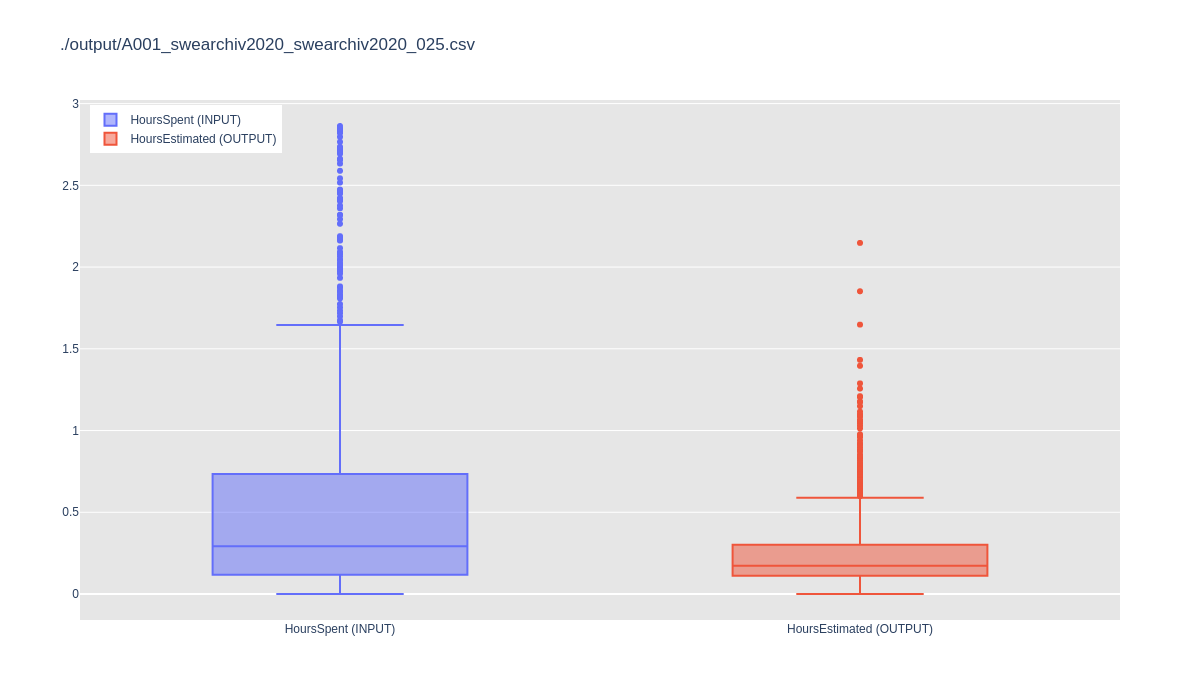
\includegraphics[width=\textwidth]{Scripts/output/A001_swearchiv2020_swearchiv2020_025.csv.png}
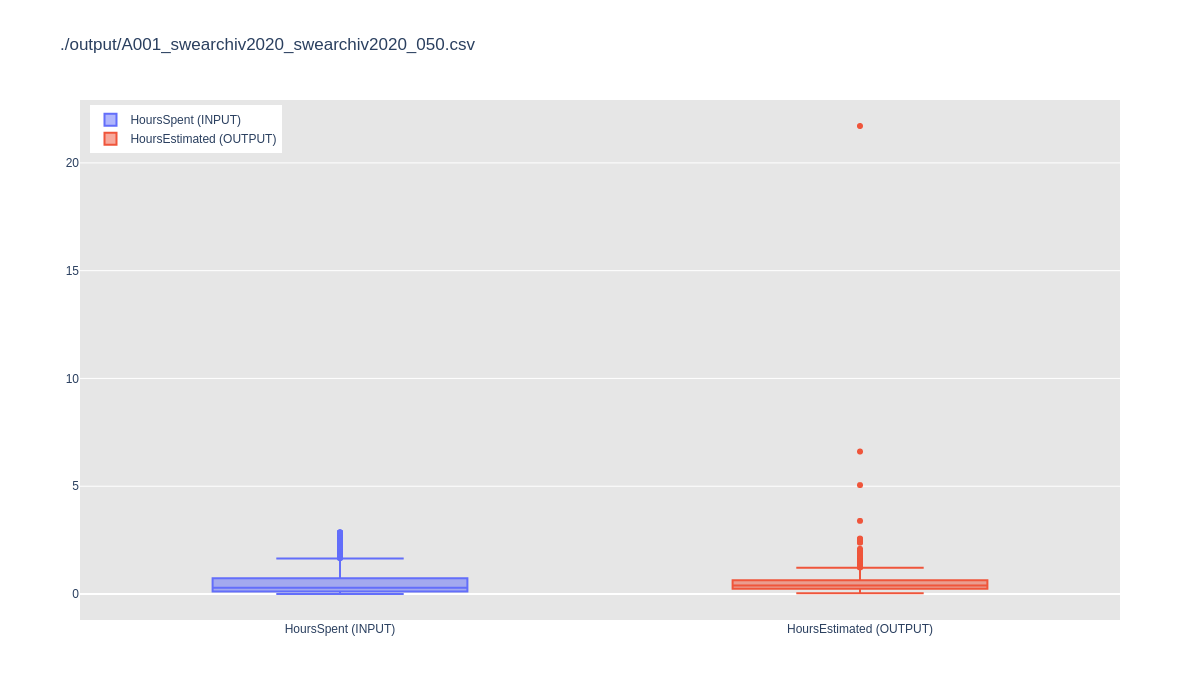
\includegraphics[width=\textwidth]{Scripts/output/A001_swearchiv2020_swearchiv2020_050.csv.png}
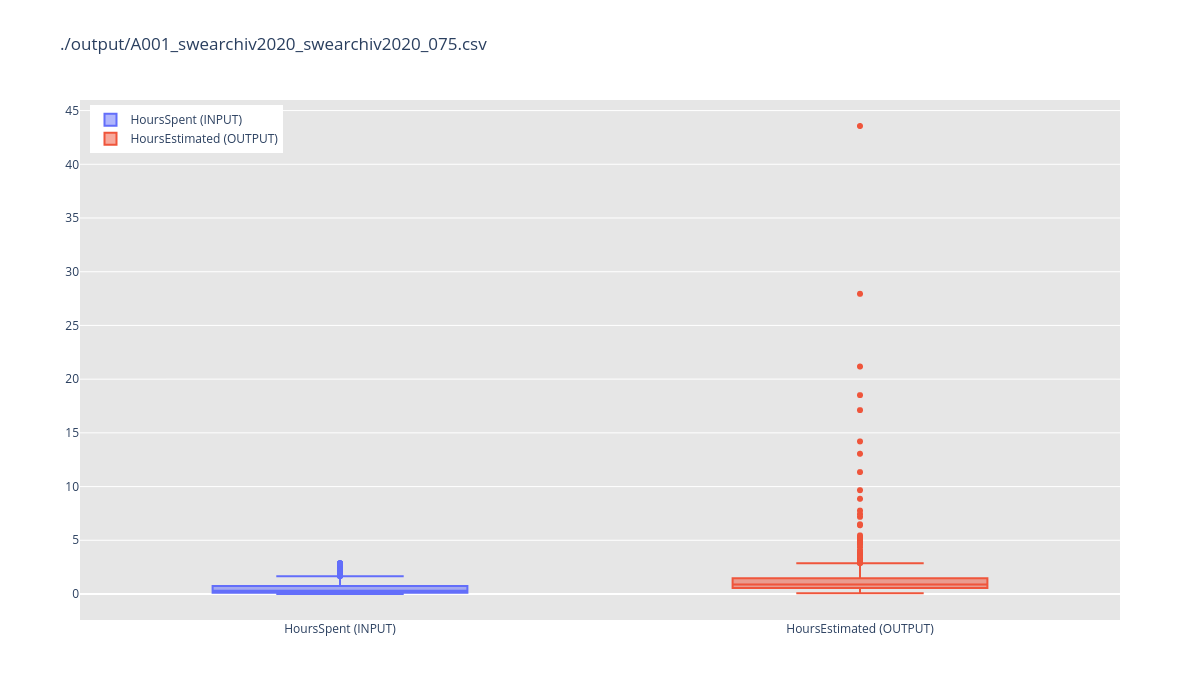
\includegraphics[width=\textwidth]{Scripts/output/A001_swearchiv2020_swearchiv2020_075.csv.png}
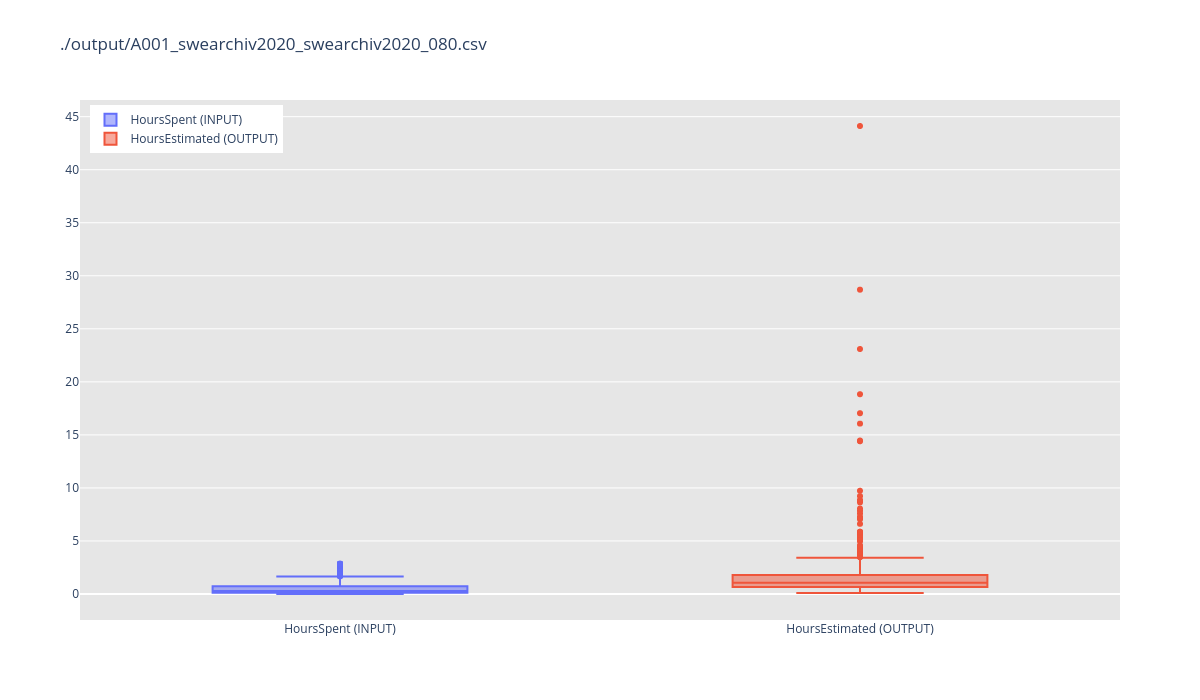
\includegraphics[width=\textwidth]{Scripts/output/A001_swearchiv2020_swearchiv2020_080.csv.png}
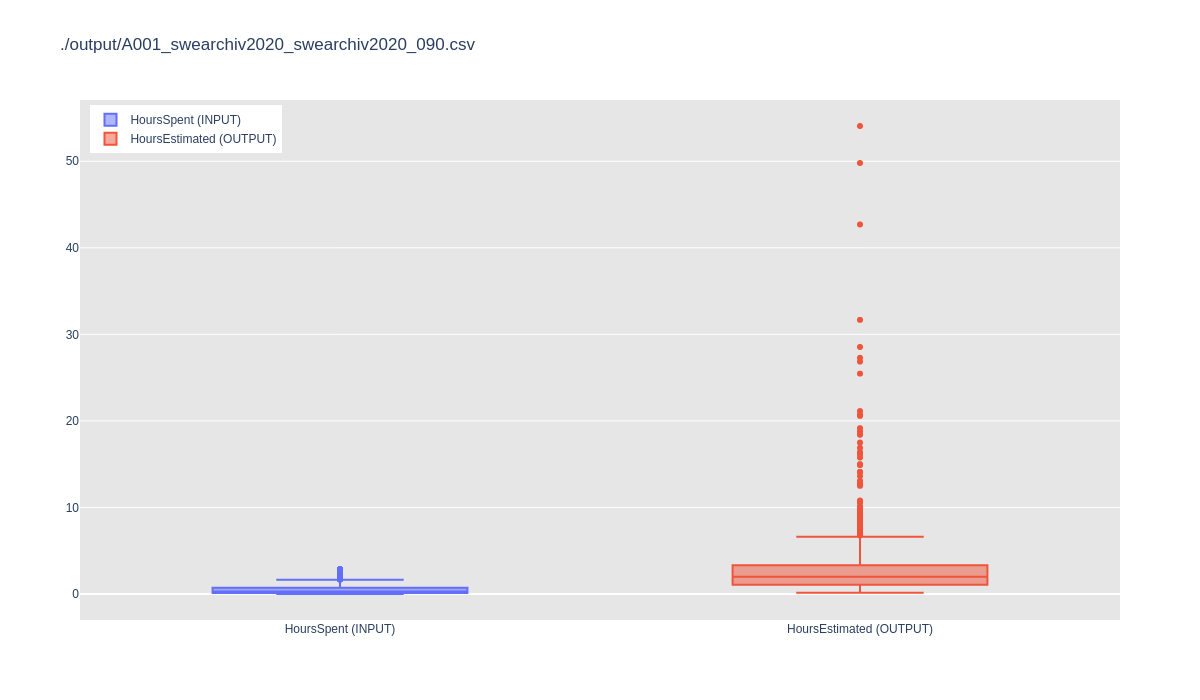
\includegraphics[width=\textwidth]{Scripts/output/A001_swearchiv2020_swearchiv2020_090.csv.png}
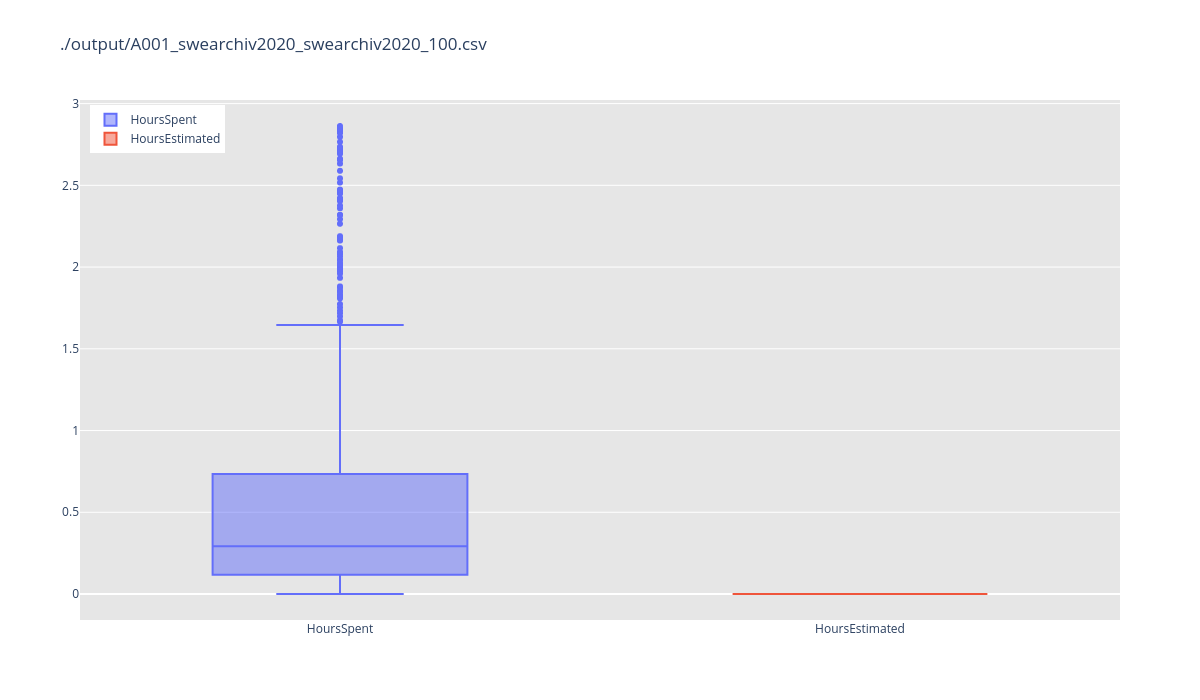
\includegraphics[width=\textwidth]{Scripts/output/A001_swearchiv2020_swearchiv2020_100.csv.png}
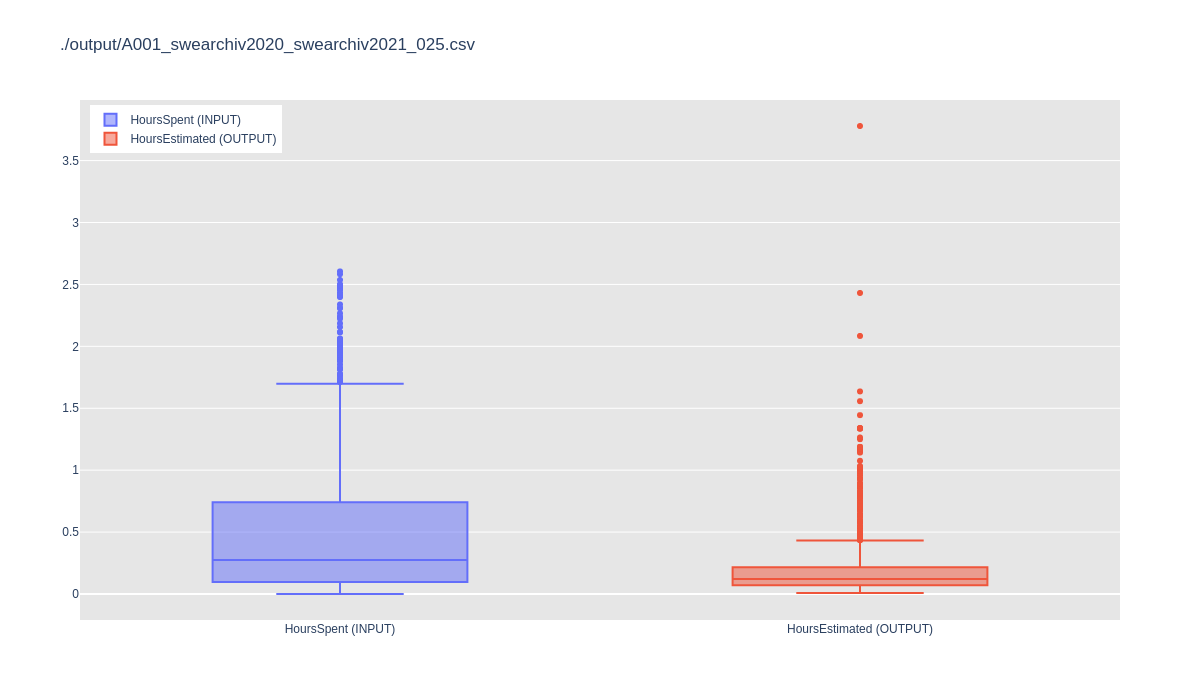
\includegraphics[width=\textwidth]{Scripts/output/A001_swearchiv2020_swearchiv2021_025.csv.png}
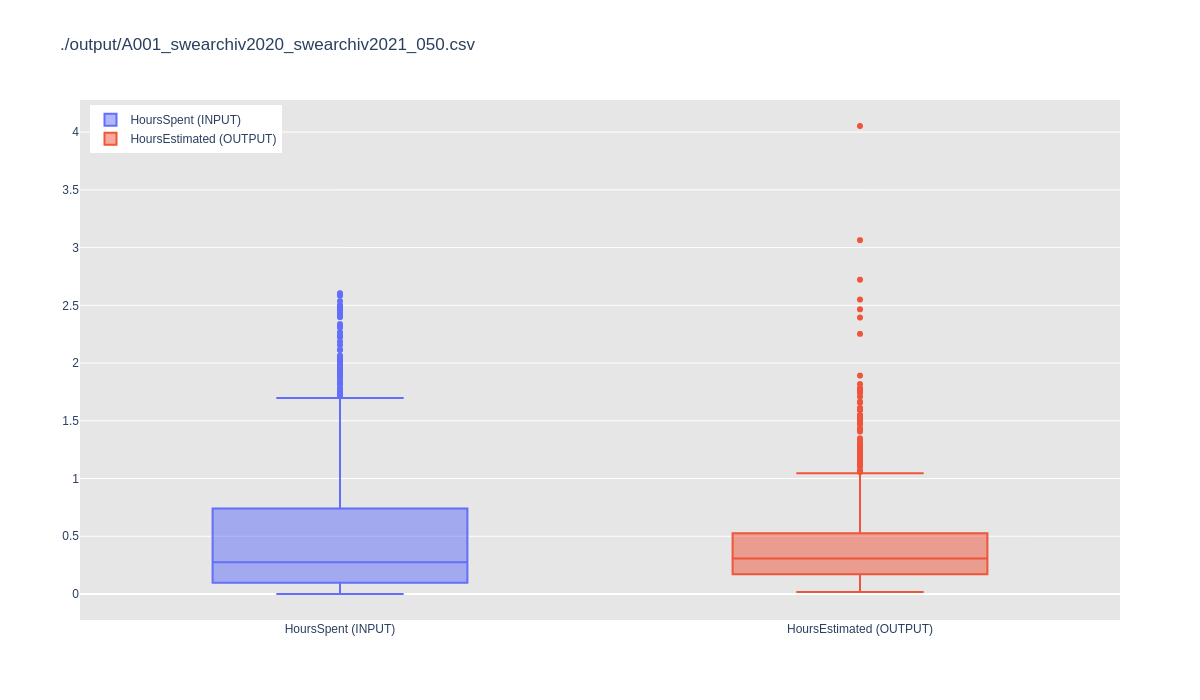
\includegraphics[width=\textwidth]{Scripts/output/A001_swearchiv2020_swearchiv2021_050.csv.png}
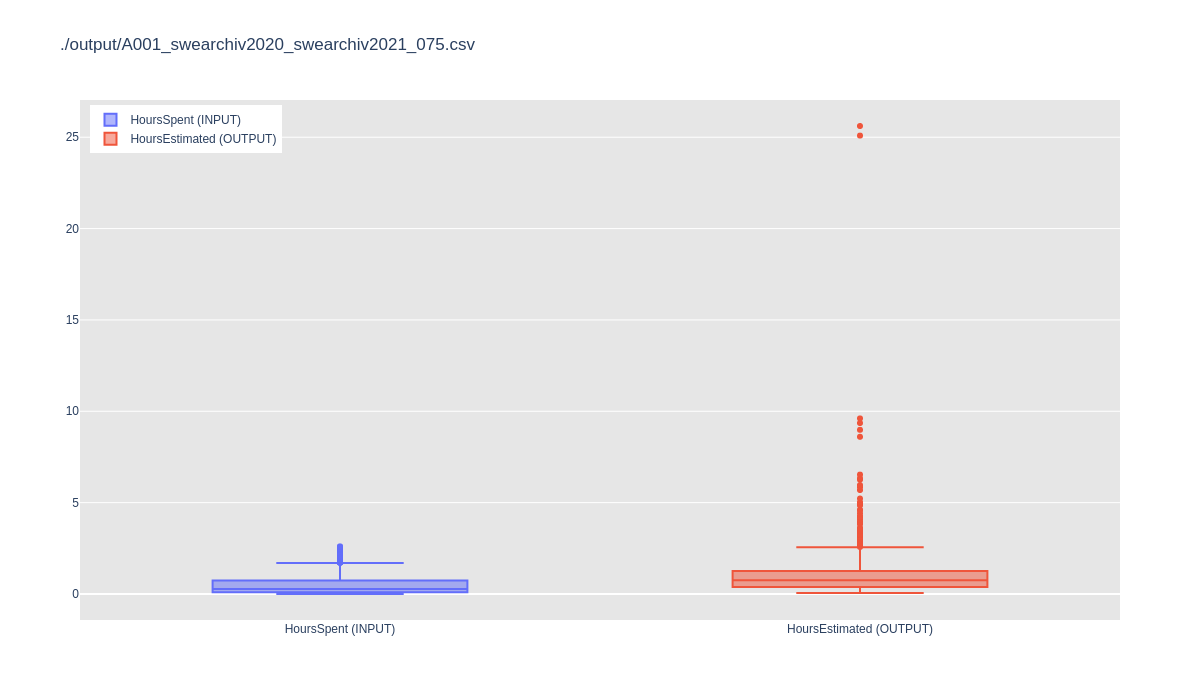
\includegraphics[width=\textwidth]{Scripts/output/A001_swearchiv2020_swearchiv2021_075.csv.png}
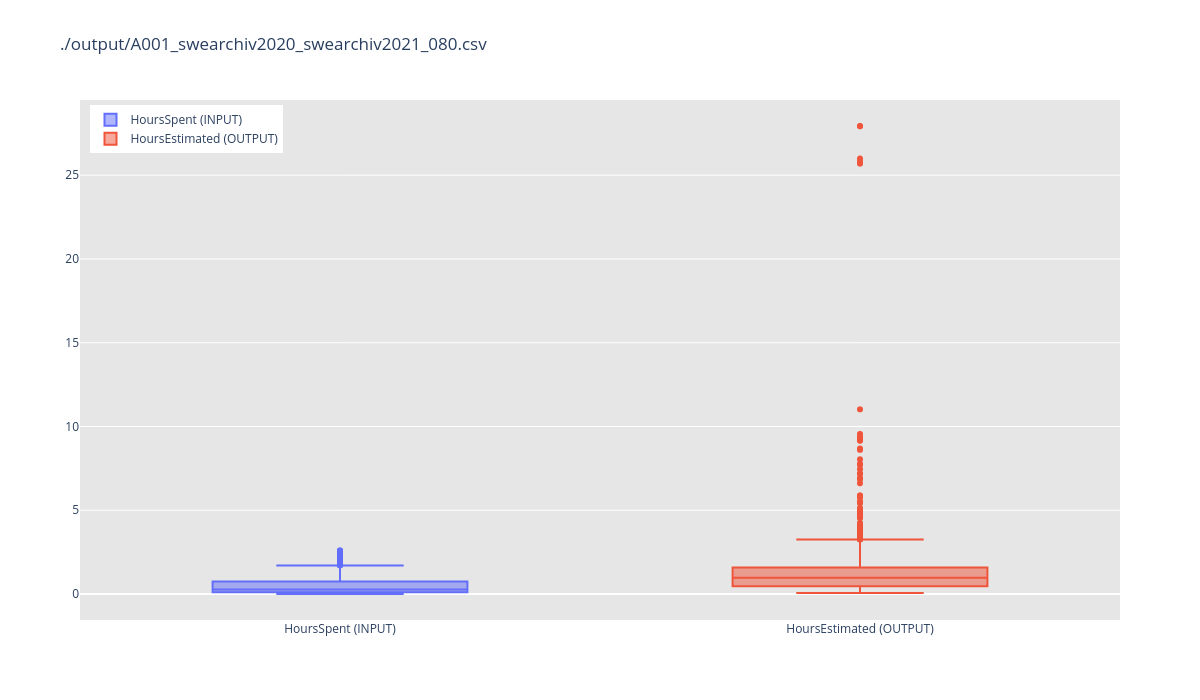
\includegraphics[width=\textwidth]{Scripts/output/A001_swearchiv2020_swearchiv2021_080.csv.png}
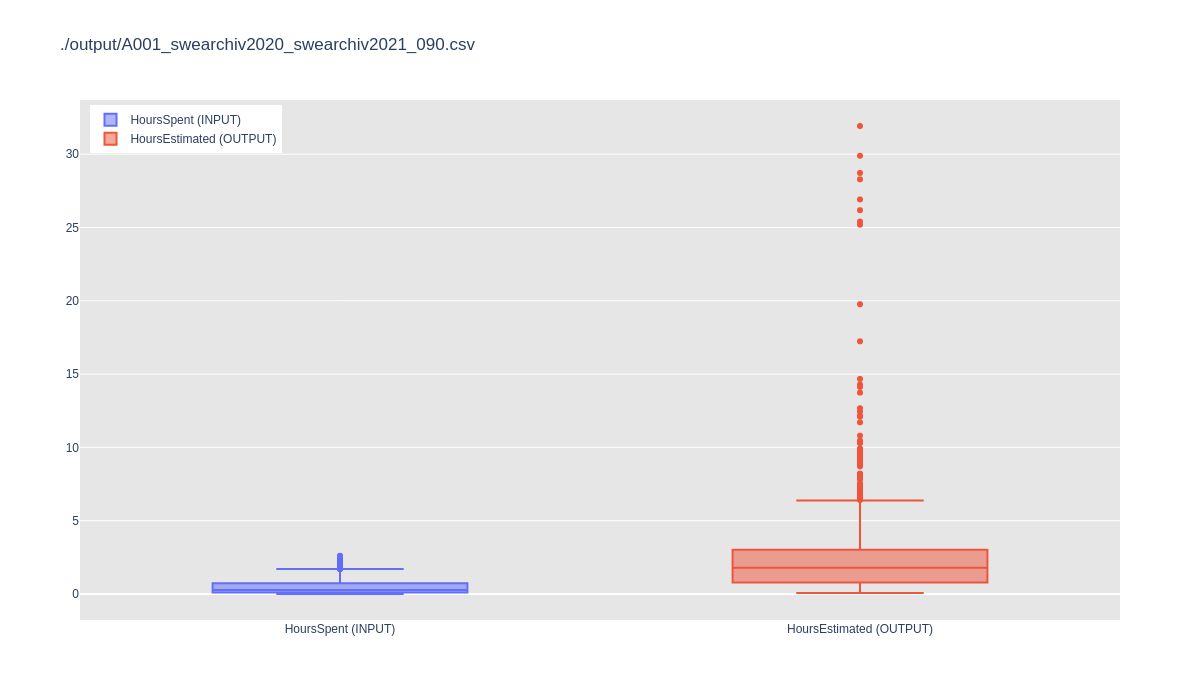
\includegraphics[width=\textwidth]{Scripts/output/A001_swearchiv2020_swearchiv2021_090.csv.png}
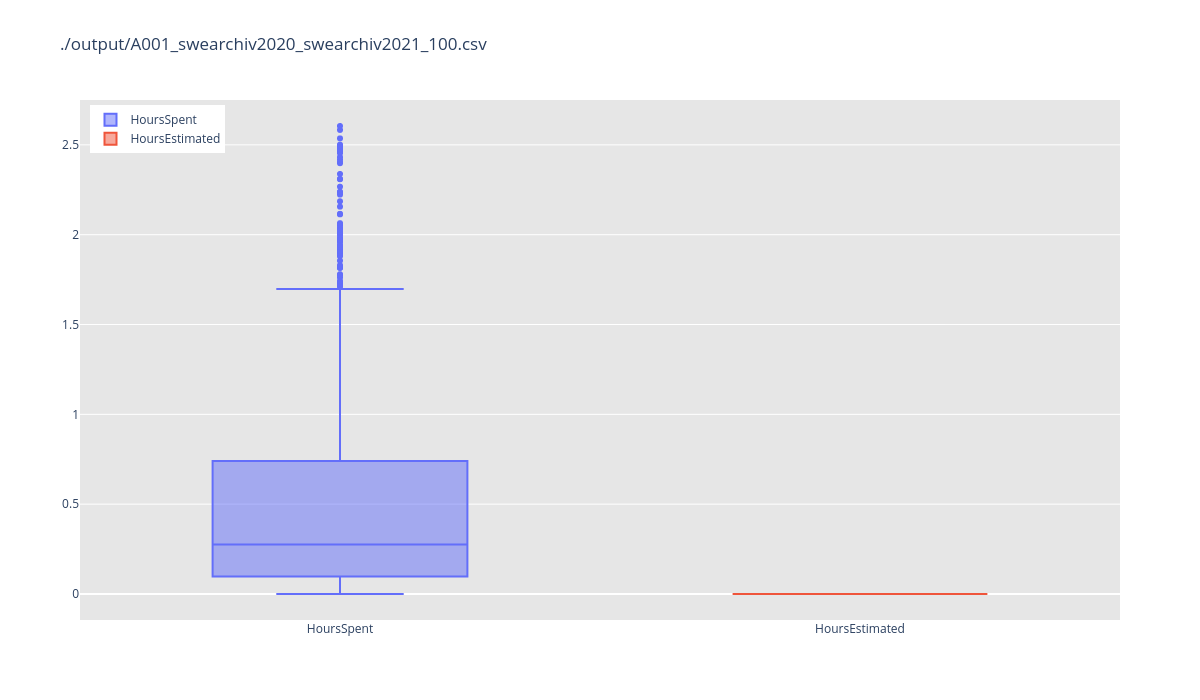
\includegraphics[width=\textwidth]{Scripts/output/A001_swearchiv2020_swearchiv2021_100.csv.png}




